% Section content template for individual Educative lessons
% This file contains the actual content for a specific section
% Generated from Educative API section content

% Section: Rate Limiter Algorithms
% Section ID: 5447913559293952
% Section Slug: rate-limiter-algorithms
% Generated: 2025-12-07T21:30:41.547415

\subsection{Algorithms for rate limiting}\label{DaVuByHkKpJOEyUdmyU5g}
\\
The task of a rate limiter is directed by highly efficient algorithms, each of which has distinct advantages and disadvantages. However, there is always a choice to choose an algorithm or combination of algorithms depending on what we need at a given time. While different algorithms are used in addition to those below, we'll take a look at the following popular algorithms.

\begin{itemize}
\item
\protect\phantomsection\label{OHUB-zXnSNRLqbDJe35_2}
Token bucket
\item
\protect\phantomsection\label{Tfyly-58W51zuahc6cZaC}
Leaking bucket
\item
\protect\phantomsection\label{CfzcXfvLHk0ZbWGzkCu_M}
Fixed window counter
\item
\protect\phantomsection\label{U90Q4DX71zwvTBdDXfKGw}
Sliding window log
\item
\protect\phantomsection\label{plnwk1Y8bNxl1HceQPff-}
Sliding window counter
\end{itemize}

\subsubsection{Token bucket algorithm}\label{KPVCOyQb7_Nhfk0nBISsB}
\\
This algorithm uses the analogy of a bucket with a predefined capacity of tokens. The bucket is periodically filled with tokens at a constant rate. A token can be considered as a packet of some specific size. Hence , the algorithm checks for the token in the bucket each time we receive a request. There should be at least one token to process the request further.
\\
The flow of the token bucket algorithm is as follows:
\\
Assume that we have a predefined rate limit of \protect\phantomsection\label{katex_inline_6id3VgfRGpUqUSgvYZxDp}{{{\(\text{R}\)}}} and the total capacity of the bucket is \protect\phantomsection\label{katex_inline_HIxbcGzVePpKk2IV9yPvA}{{{\(\text{C}\)}}}.

\begin{enumerate}
\item
\protect\phantomsection\label{ZNbr0uPVUqo9fC2kBP28G}
The algorithm adds a new token to the bucket after every R1\hspace{0pt} seconds.
\item
\protect\phantomsection\label{gua4YXBWU72fG6VtFZJ4q}
The algorithm discards the new incoming tokens when the number of tokens in the bucket is equal to the total capacity C of the bucket.
\item
\protect\phantomsection\label{4GTGo55s7Txa0g6GdJPp7}
If there are N incoming requests and the bucket has at least N tokens, the tokens are consumed, and requests are forwarded for further processing.
\item
\protect\phantomsection\label{CqAwXZrEUUC_nkcHQTNcG}
If there are N incoming requests and the bucket has a lower number of tokens, then the number of requests accepted equals the number of available tokens in the bucket.
\end{enumerate}
\\
The following illustration represents the working of the token bucket algorithm.

\begin{figure}[htbp]
 \centering
 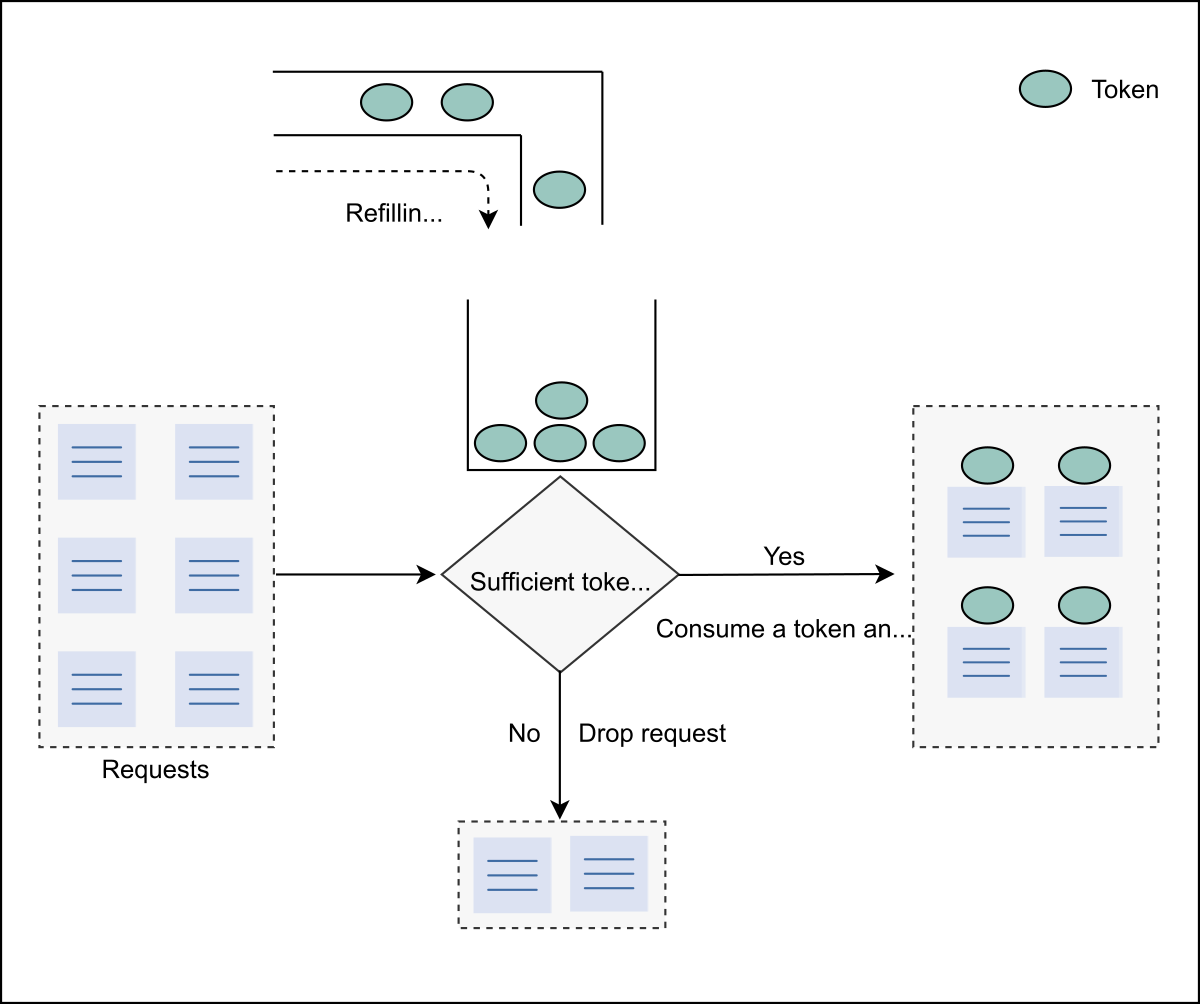
\includegraphics[width=0.5\textwidth]{Images/chapter_19/section_5447913559293952/5992337486643200.png}
 \caption{How the token bucket algorithm works}
\end{figure}

The following illustration demonstrates how token consumption and rate-limiting logic work. In this example, the capacity of the bucket is three, and it is refilled at a rate of three tokens per minute.

\begin{figure}[htbp]
 \centering
 \begin{subfigure}[b]{0.48\textwidth}
 \centering
 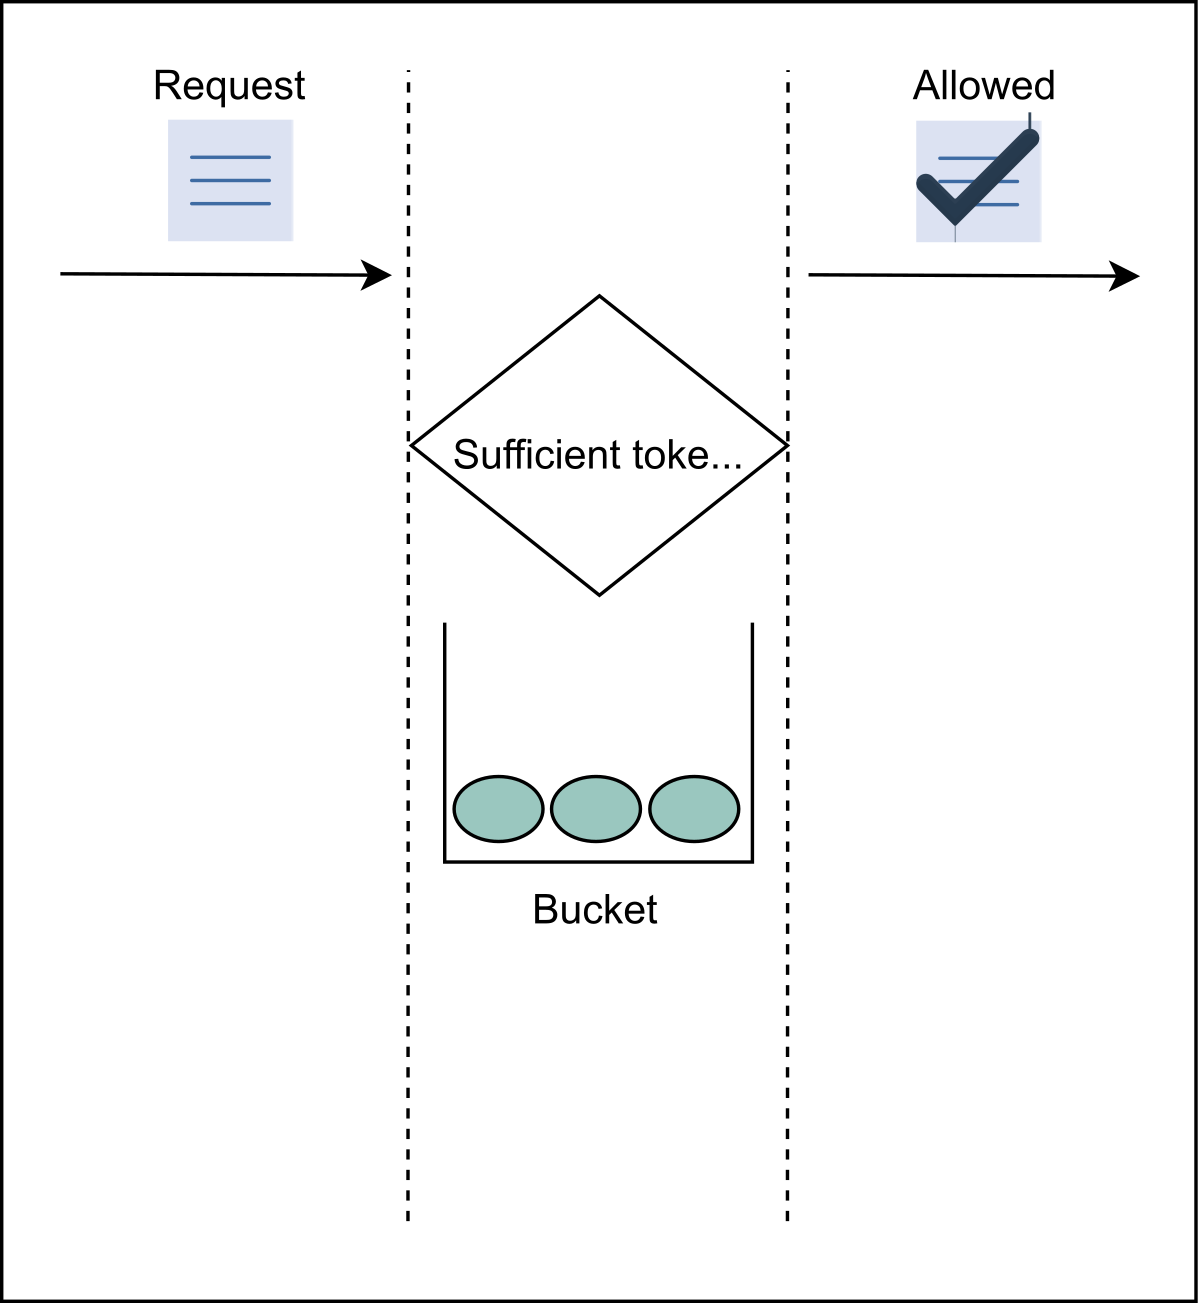
\includegraphics[width=\textwidth]{Images/chapter_19/section_5447913559293952/5222201733414912.png}
 \caption{Initially, there are three tokens in the bucket. A request arrives within a minute and consumes a token from the bucket}
 \end{subfigure}
 \hfill
 \begin{subfigure}[b]{0.48\textwidth}
 \centering
 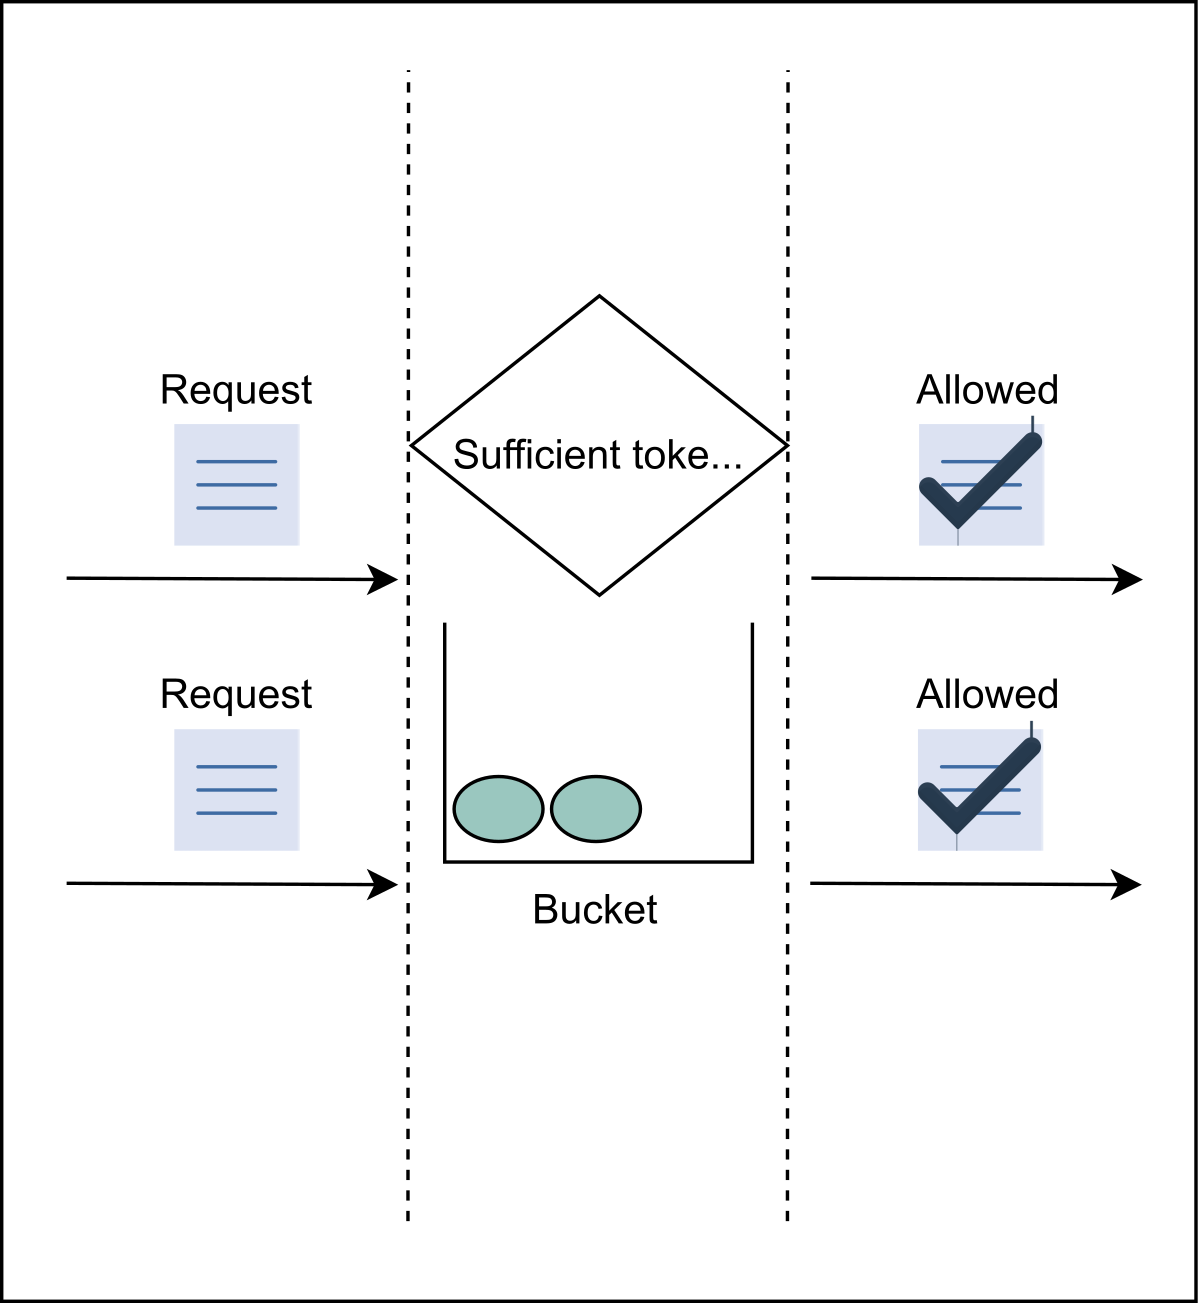
\includegraphics[width=\textwidth]{Images/chapter_19/section_5447913559293952/5365267463143424.png}
 \caption{Two more request within same minute arrive and consume the remaining two tokens }
 \end{subfigure}
\end{figure}

\begin{figure}[htbp]
 \centering
 \begin{subfigure}[b]{0.48\textwidth}
 \centering
 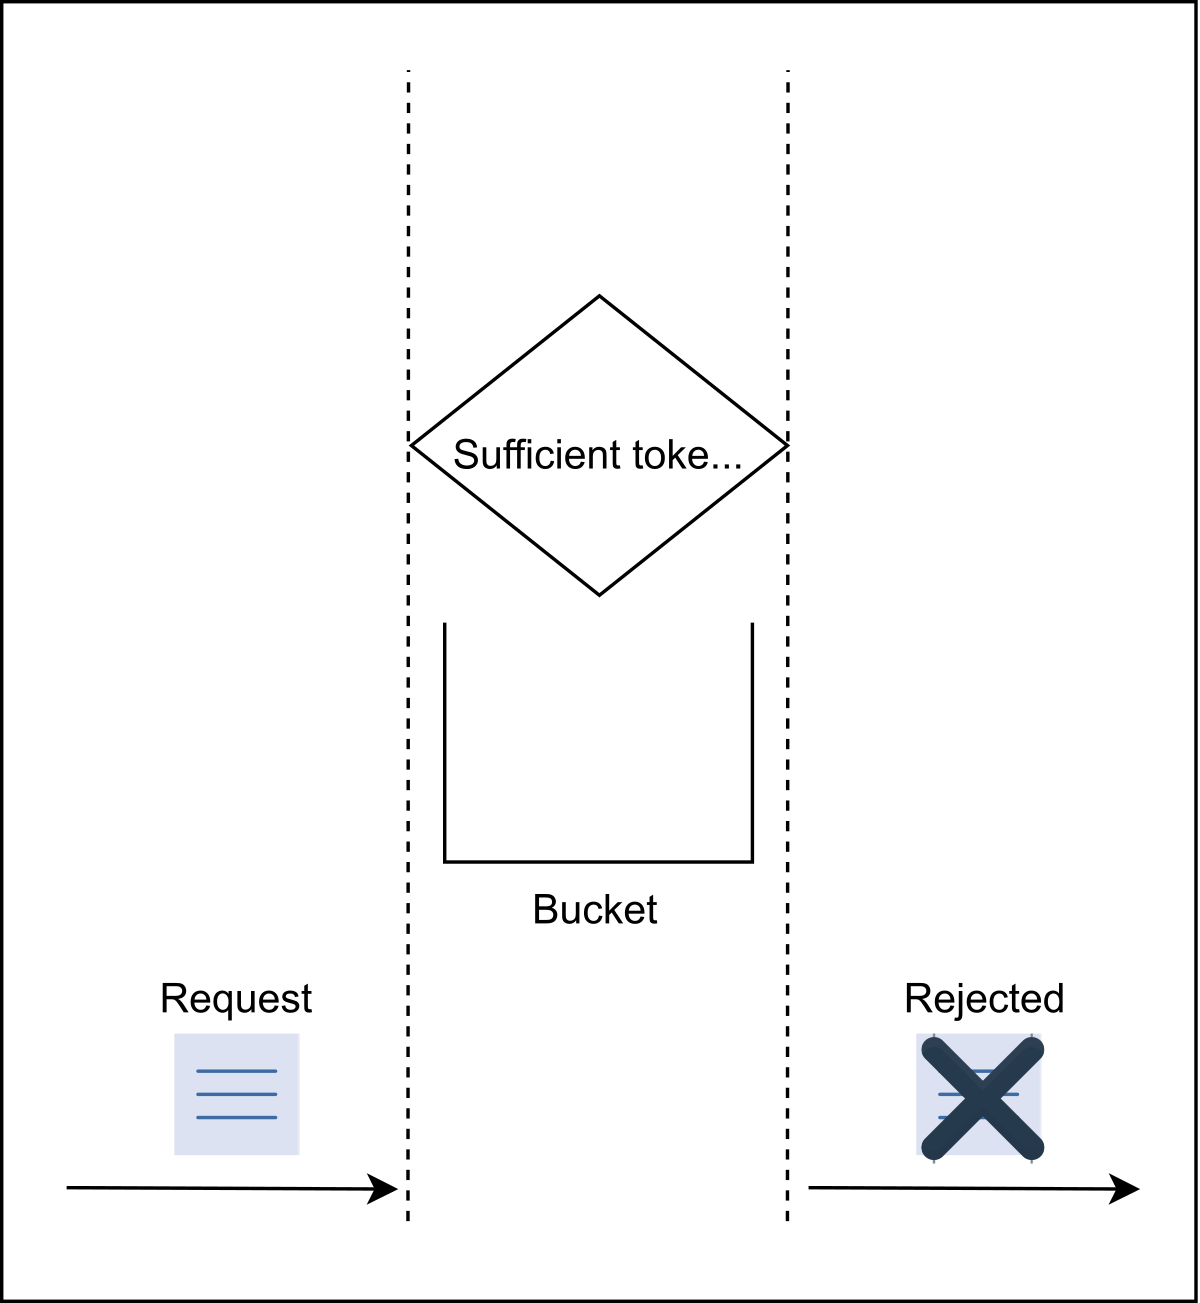
\includegraphics[width=\textwidth]{Images/chapter_19/section_5447913559293952/4694045041623040.png}
 \caption{One more (fourth) request arrives in the same minute. Reject the request because the bucket is empty}
 \end{subfigure}
 \hfill
 \begin{subfigure}[b]{0.48\textwidth}
 \centering
 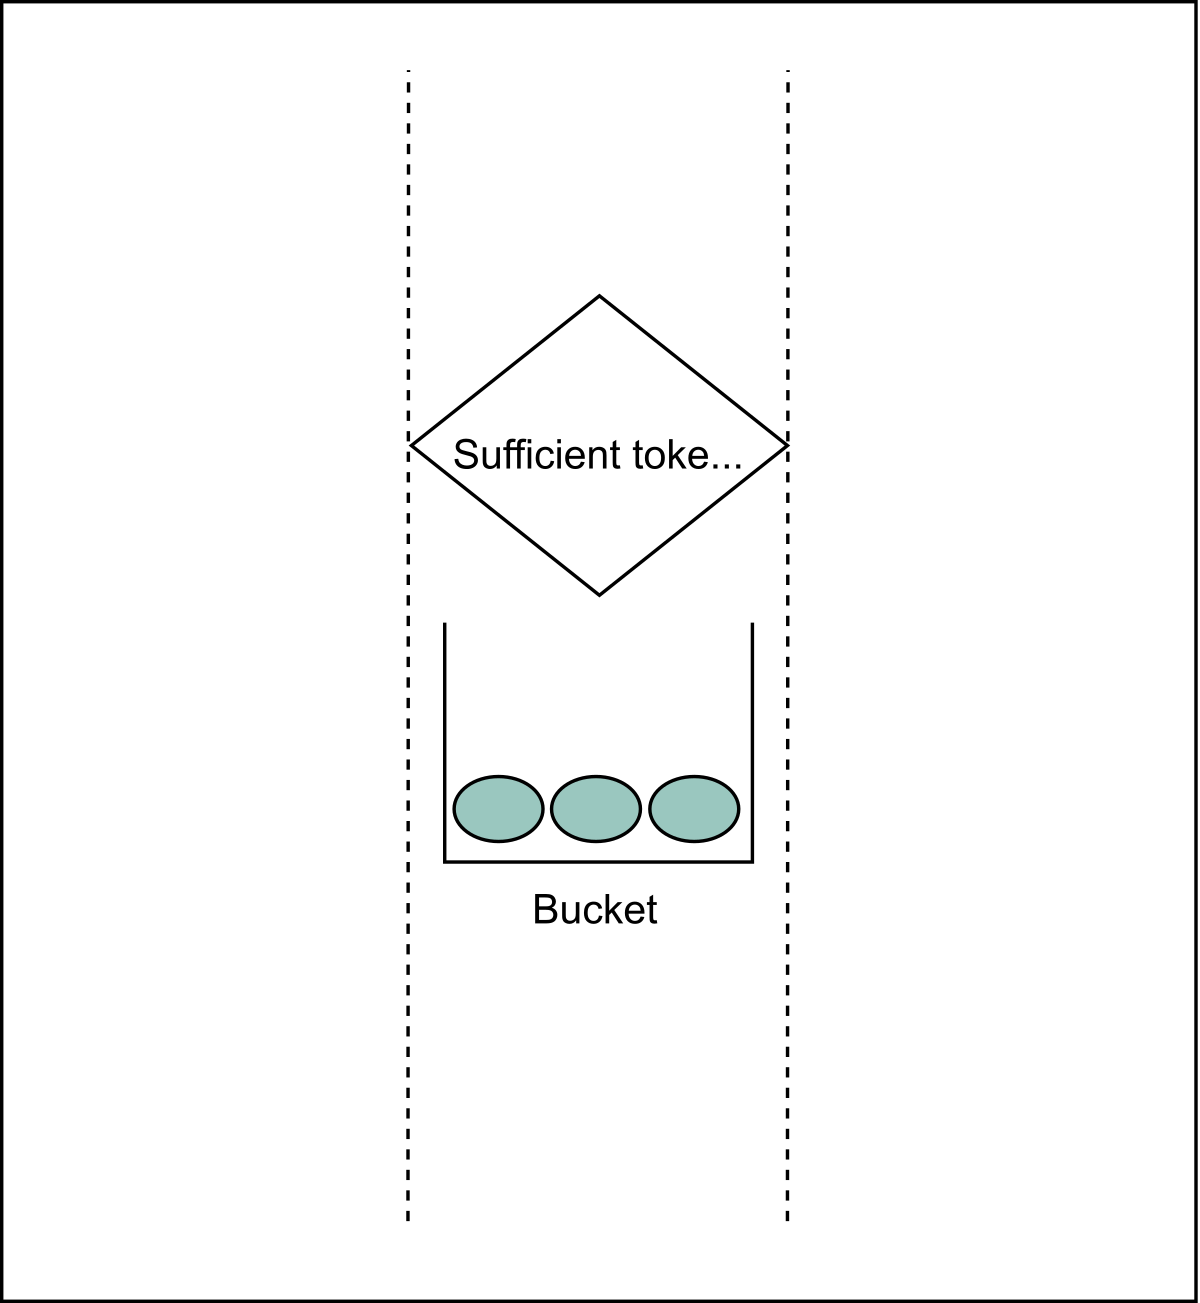
\includegraphics[width=\textwidth]{Images/chapter_19/section_5447913559293952/6094055130005504.png}
 \caption{Refill the bucket after one minute}
 \end{subfigure}
\end{figure}

\paragraph{Essential parameters}\label{ciLz-7N5CCGQSz3Cho0NX}
\\
We require the following essential parameters to implement the token bucket algorithm:

\begin{itemize}
\item
\protect\phantomsection\label{gTJr7msrq4R-qlnxZtiEw}
\textbf{Bucket capacity} \protect\phantomsection\label{katex_inline_BYQ9tRwfP-p5To3cSoz_y}{{{\((\text{C})\)}}}: The maximum number of tokens that can reside in the bucket.
\item
\protect\phantomsection\label{r6IVPeKwnEPL8zj-5fUPh}
\textbf{Rate limit} \protect\phantomsection\label{katex_inline_rPm2AVIRLxwWsrqUtjfV_}{{{\((\text{R})\)}}}\textbf{:} The number of requests we want to limit per unit time.
\item
\protect\phantomsection\label{z-dpWZ8PWp_uo1AQcKrGu}
\textbf{Refill rate} \protect\phantomsection\label{katex_inline_iaRKBeWmmv3r9uEdkwfaP}{{{\((\frac{1}{\text{R}})\)}}}\textbf{:} The duration after which a token is added to the bucket.
\item
\protect\phantomsection\label{KqJ-HOAF_78Q395G0aQsb}
\textbf{Requests count} \protect\phantomsection\label{katex_inline_cgXtaaEHX-IN57hbyZ8jF}{{{\((\text{N})\)}}}\textbf{:} This parameter tracks the number of incoming requests and compares them with the bucket's capacity.
\end{itemize}
\\
\paragraph{Advantages}\label{5ZBoq-KXWaWnovjrxxzm7}

\begin{itemize}
\item
\protect\phantomsection\label{xspT09l539PFnGknVKGna}
This algorithm can cause a burst of traffic as long as there are enough tokens in the bucket.
\item
\protect\phantomsection\label{7mEUNKmAqIR75e_qO_e2W}
It is space efficient. The memory needed for the algorithm is nominal due to limited states.
\end{itemize}
\\
\paragraph{Disadvantages}\label{wntOhM5RHY_oE6ZB6_wfj}

\begin{itemize}
\item
\protect\phantomsection\label{C12WkYi8WpS8iT7DBdzXQ}
Choosing an optimal value for the essential parameters is a difficult task.
\end{itemize}

\begin{quote}
\textbf{Quiz:}
\textbf{Question 1:} Apart from permitting bursts, can the token bucket algorithm surpass the limit at the edges?
\textbf{Answer:} Yes, the token bucket algorithm can sometimes suffer from overrunning the limit at the edges, as demonstrated by the following example:

Consider a scenario with a bucket capacity equal to \$3\$, and the number of requests allowed per minute is also \$3\$. This yields a refill rate of \$0.33\$ minutes, which means that a new token will come every \$0.33\$ minute. In the illustration below, three tokens have been accumulated at the end of the first minute. At the same time, a burst of requests arrives and consumes all three tokens, leaving the bucket empty. At the end of \$1.33\$ minutes (at a refill rate of \$0.33\$), a new token is added to the bucket. Simultaneously, a new request arrives and consumes the token. However, if we consider the duration from

\$0.66\$ to \$1.33\$ minutes, we\textquotesingle ll see that a total of four tokens have been consumed. This example shows that the token bucket can surpass the limit at the edges.

\end{quote}

\subsubsection{The leaking bucket algorithm}\label{TwLqXyqBxH25au8fRMtUq}
\\
The \textbf{leaking bucket algorithm} is a variant of the token bucket algorithm with slight modifications. Instead of using tokens, the leaking bucket algorithm uses a bucket to contain incoming requests and processes them at a constant outgoing rate. This algorithm uses the analogy of a water bucket leaking at a constant rate. Similarly, in this algorithm, the requests arrive at a variable rate. The algorithm process these requests at a constant rate in a first-in-first-out (FIFO) order.
\\
Let's look at how the leaking bucket algorithm works in the illustration below:

\begin{figure}[htbp]
 \centering
 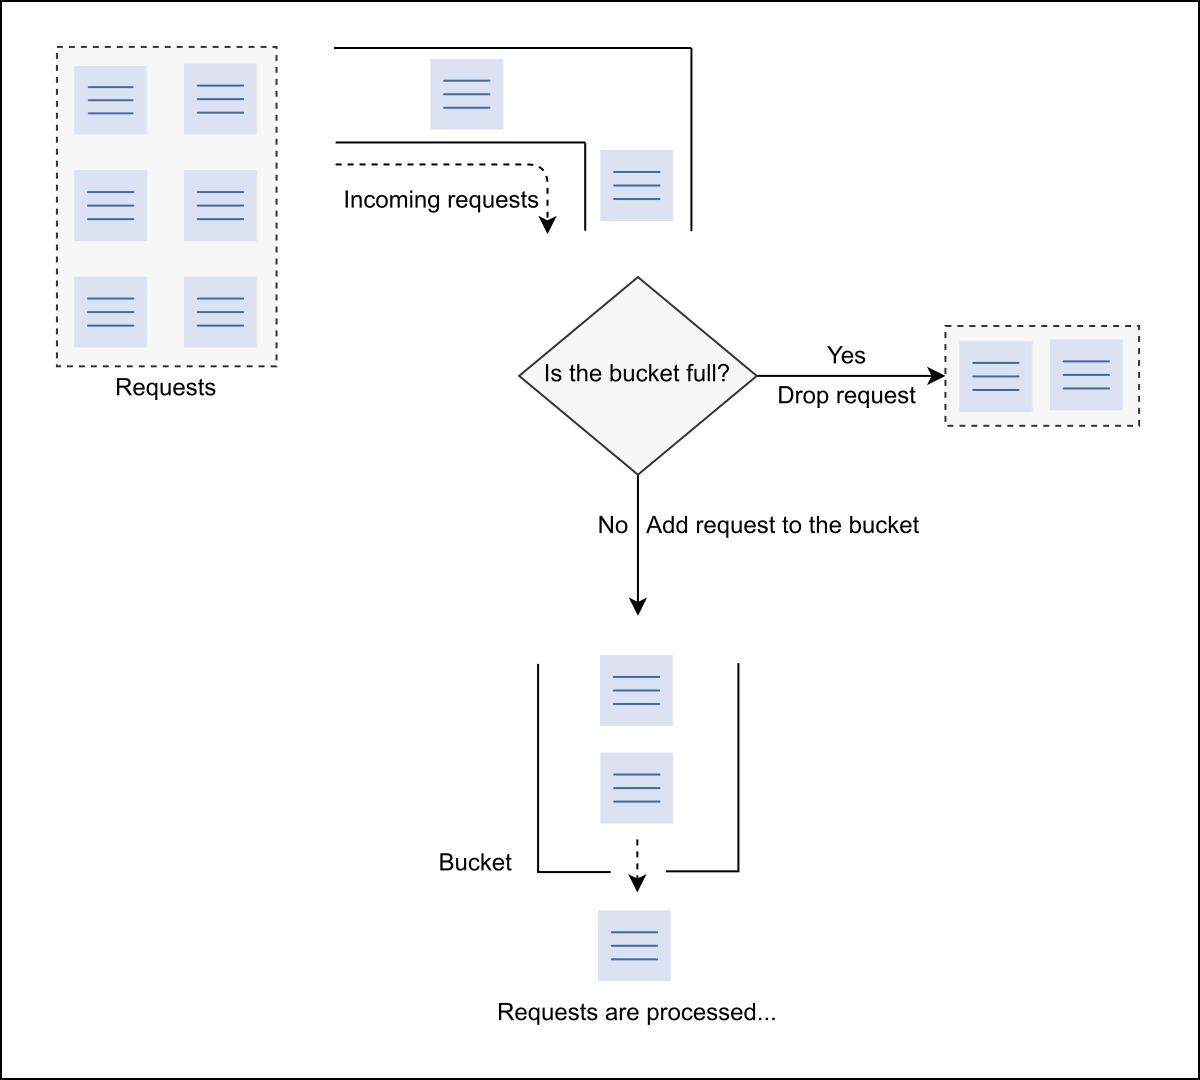
\includegraphics[width=0.5\textwidth]{Images/chapter_19/section_5447913559293952/6605449973727232.png}
 \caption{How the leaking bucket algorithm works}
\end{figure}

\paragraph{Essential parameters}\label{VZsS_2buJoI4klQKLCBMa}
\\
The leaking bucket algorithm requires the following parameters.

\begin{itemize}
\item
\protect\phantomsection\label{UzGu46415BTDD9UcnUKkO}
\textbf{Bucket capacity} \protect\phantomsection\label{katex_inline_axP4q-n0DaIE--aXXn0hY}{{{\(\text{(C)}\)}}}\textbf{:} This determines the maximum capacity of the bucket. The algorithm will discard the incoming requests when the bucket reached its maximum limit of \protect\phantomsection\label{katex_inline_AX90pse8YMIE2ljHhKDqh}{{{\(\text{C}\)}}}.
\item
\protect\phantomsection\label{g3h9pfIEEzO28n6QLmpea}
\textbf{Inflow rate} \protect\phantomsection\label{katex_inline_O6UCCWh4bFO0dbK6cXxjP}{{{\(\text{(R}_\text{{in}})\)}}}\textbf{:} This parameter shows the inflow rate of requests. This is a varying quantity that depends on the application and nature of requests. We use this parameter to find the initial capacity of the bucket.
\item
\protect\phantomsection\label{EUbzh8wtZd6AuIGBXpQfU}
\textbf{Outflow rate} \protect\phantomsection\label{katex_inline_dJGbkIeTBiI1D0lUowXCN}{{{\(\text{(R}_\text{{out}})\)}}}\textbf{:} This determines the number of requests processed per unit time.
\end{itemize}
\\
\paragraph{Advantages}\label{PYA2L903Pd2o6LUipvpGF}

\begin{itemize}
\item
\protect\phantomsection\label{pP0y6AjjRwwh02OFpOAgy}
Due to a constant outflow rate (\protect\phantomsection\label{katex_inline_AFeSwv1cg6PhnQypICaRC}{{{\(\text{R}_\text{{out​}}\)}}}), it avoids the burst of requests, unlike the token bucket algorithm.
\item
\protect\phantomsection\label{k_xNe0X_LIHHS7APata7N}
This algorithm is also space efficient since it requires just three states: inflow rate \protect\phantomsection\label{katex_inline_Xvc8ZPFL5_b5kVakdHJ6i}{{{\(\text{(R}_\text{{in​}})\)}}}, outflow rate \protect\phantomsection\label{katex_inline_rbLOepA_Ls12RwIKT6xEv}{{{\(\text{(R}_\text{{in​}})\)}}}, and bucket capacity \protect\phantomsection\label{katex_inline_cN_20aRoTL40mtQK3rglj}{{{\(\text{(C)}\)}}}.
\item
\protect\phantomsection\label{kefLGQu5cksFSsqY_Pj1M}
Since requests are processed at a fixed rate, it is suitable for applications with a stable outflow rate.
\end{itemize}
\\
\paragraph{Disadvantages}\label{X8il33JuIhG9WJV_ftkEy}

\begin{itemize}
\item
\protect\phantomsection\label{BMDKOzIsXlDoiKV_fGlAz}
A burst of requests can fill the bucket, and if not processed in the specified time, recent requests can take a hit.
\item
\protect\phantomsection\label{u_eUp9Sx2fqF_40zRrtcE}
Determining an optimal bucket size and outflow rate is a challenge.
\end{itemize}

\subsubsection{Fixed window counter algorithm}\label{gon2Zrghw-96wFgXvrocm}
\\
This algorithm divides the time into fixed intervals called \textbf{windows} and assigns a counter to each window. When a specific window receives a request, the counter is incremented by one. Once the counter reaches its limit, new requests are discarded in that window.
\\
As shown in the below figure, a dotted line represents the limit in each window. If the counter is lower than the limit, forward the request; otherwise, discard the request.

\begin{figure}[htbp]
 \centering
 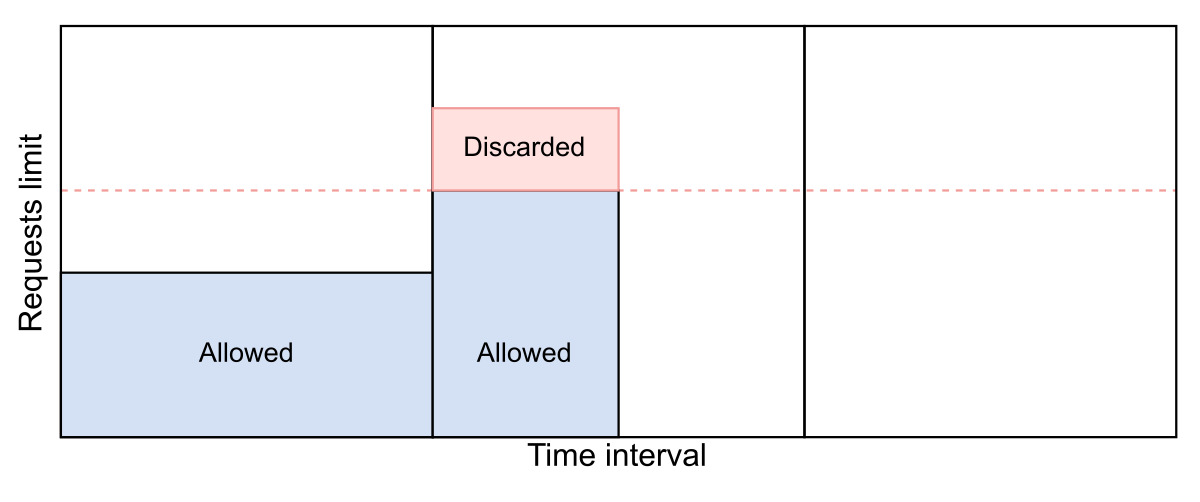
\includegraphics[width=0.5\textwidth]{Images/chapter_19/section_5447913559293952/5752531276005376.png}
 \caption{Fixed window counter algorithm: Discard the request exceeding the limit }
\end{figure}

There is a significant problem with this algorithm. A burst of traffic greater than the allowed requests can occur at the edges of the window. In the below figure, the system allows a maximum of ten requests per minute. However, the number of requests in the one-minute window from 01:30 to 02:30 is 20, which is greater than the allowed number of requests.\\

\begin{figure}[htbp]
 \centering
 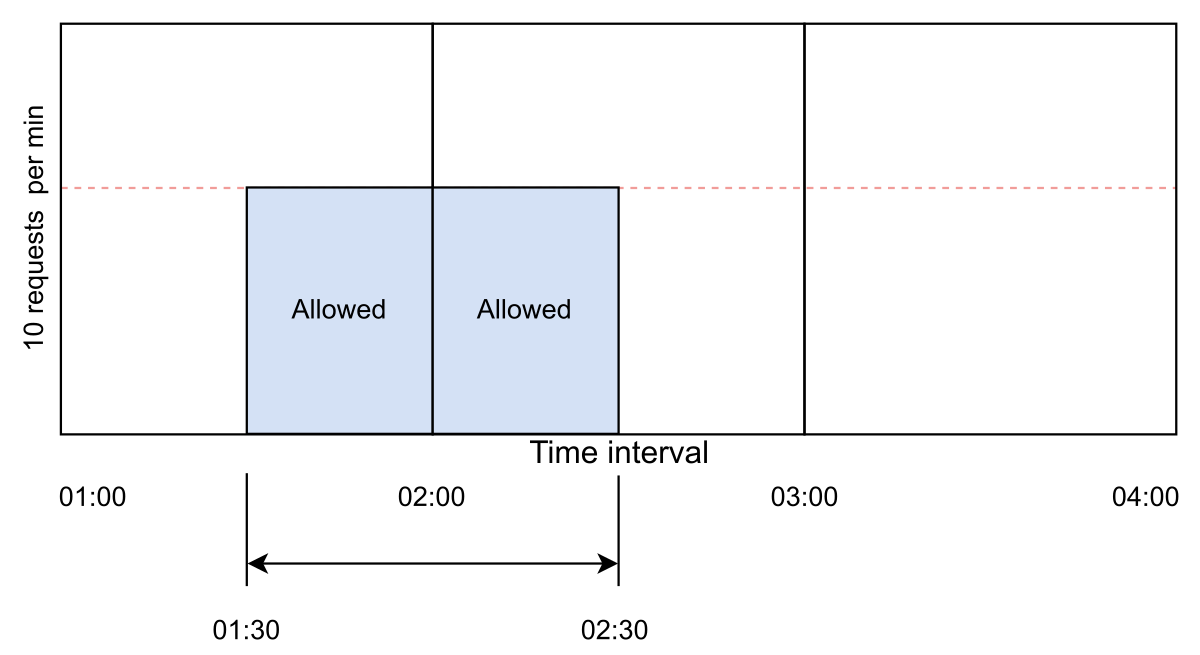
\includegraphics[width=0.5\textwidth]{Images/chapter_19/section_5447913559293952/4904797945987072.png}
 \caption{Edge case problem in the fixed window counter algorithm. The number of requests in one minute from 01:30 to 02:30 exceeds the predefined limit of 10 requests per minute}
\end{figure}

\paragraph{Essential parameters}\label{o_jzjhPkE2Nmn2XGO6dB_}
\\
The fixed window counter algorithm requires the following parameters:

\begin{itemize}
\item
\protect\phantomsection\label{Ut2MW8xqJQnV0W6WwFp8m}
\textbf{Window size} \protect\phantomsection\label{katex_inline_AoJGm2KqngJP4iTMkcTKj}{{{\(\text{(W)}\)}}}\textbf{:} It represents the size of the time window. It can be a minute, an hour, or any other suitable time slice.
\item
\protect\phantomsection\label{wzuynYC16FSJTcnzBZkF_}
\textbf{Rate limit} \protect\phantomsection\label{katex_inline_rW8AHIcz9I0FMRG_kvkG5}{{{\(\text{(R)}\)}}}: It shows the number of requests allowed per time window.
\item
\protect\phantomsection\label{vbZxYym1dC49ufUqEUHDT}
\textbf{Requests count} \protect\phantomsection\label{katex_inline_ALMzm994FUZN61UJw6qEU}{{{\(\text{(N)}\)}}}\textbf{:} This parameter shows the number of incoming requests per window. The incoming requests are allowed if \protect\phantomsection\label{katex_inline_yV6ZzXlLgMXlqV65UkBWZ}{{{\(\text{N}\)}}} is less than or equal to \protect\phantomsection\label{katex_inline_aEP9EWKupzfgnxy-_C0p6}{{{\(\text{R}\)}}}.
\end{itemize}
\\
\paragraph{Advantages}\label{TXsyd0ihhX_A0vxOHdfic}

\begin{itemize}
\item
\protect\phantomsection\label{ouL1XqbccRbFGBtJeabn7}
It is also space efficient due to constraints on the rate of requests.
\item
\protect\phantomsection\label{3c8dlvQOYX9uokCBhtmjn}
As compared to token bucket-style algorithms (that discard the new requests if there aren't enough tokens), this algorithm services the new requests.
\end{itemize}
\\
\paragraph{Disadvantages}\label{fUqha70lhnGSJ2P-wwQZB}

\begin{itemize}
\item
\protect\phantomsection\label{AZjwd7D6oKKKmCphv-0Yg}
A consistent burst of traffic (twice the number of allowed requests per window) at the window edges could cause a potential decrease in performance.
\end{itemize}

\subsubsection{Sliding window log algorithm}\label{4gFY1cUHd0C6474tFaYqH}
\\
The \textbf{sliding window log algorithm} keeps track of each incoming request. When a request arrives, its arrival time(Also known as a time stamp.) is stored in a hash map, usually known as the log. The logs are sorted based on the time stamps of incoming requests. The requests are allowed depending on the size of the log and arrival time.
\\
The main advantage of this algorithm is that it doesn't suffer from the edge conditions, as compared to the \textbf{fixed window counter} algorithm.
\\
Let's understand how the sliding window log algorithm works in the illustration below. Assume that we have a maximum rate limit of two requests in a minute.

\begin{figure}[htbp]
 \centering
 \begin{subfigure}[b]{0.48\textwidth}
 \centering
 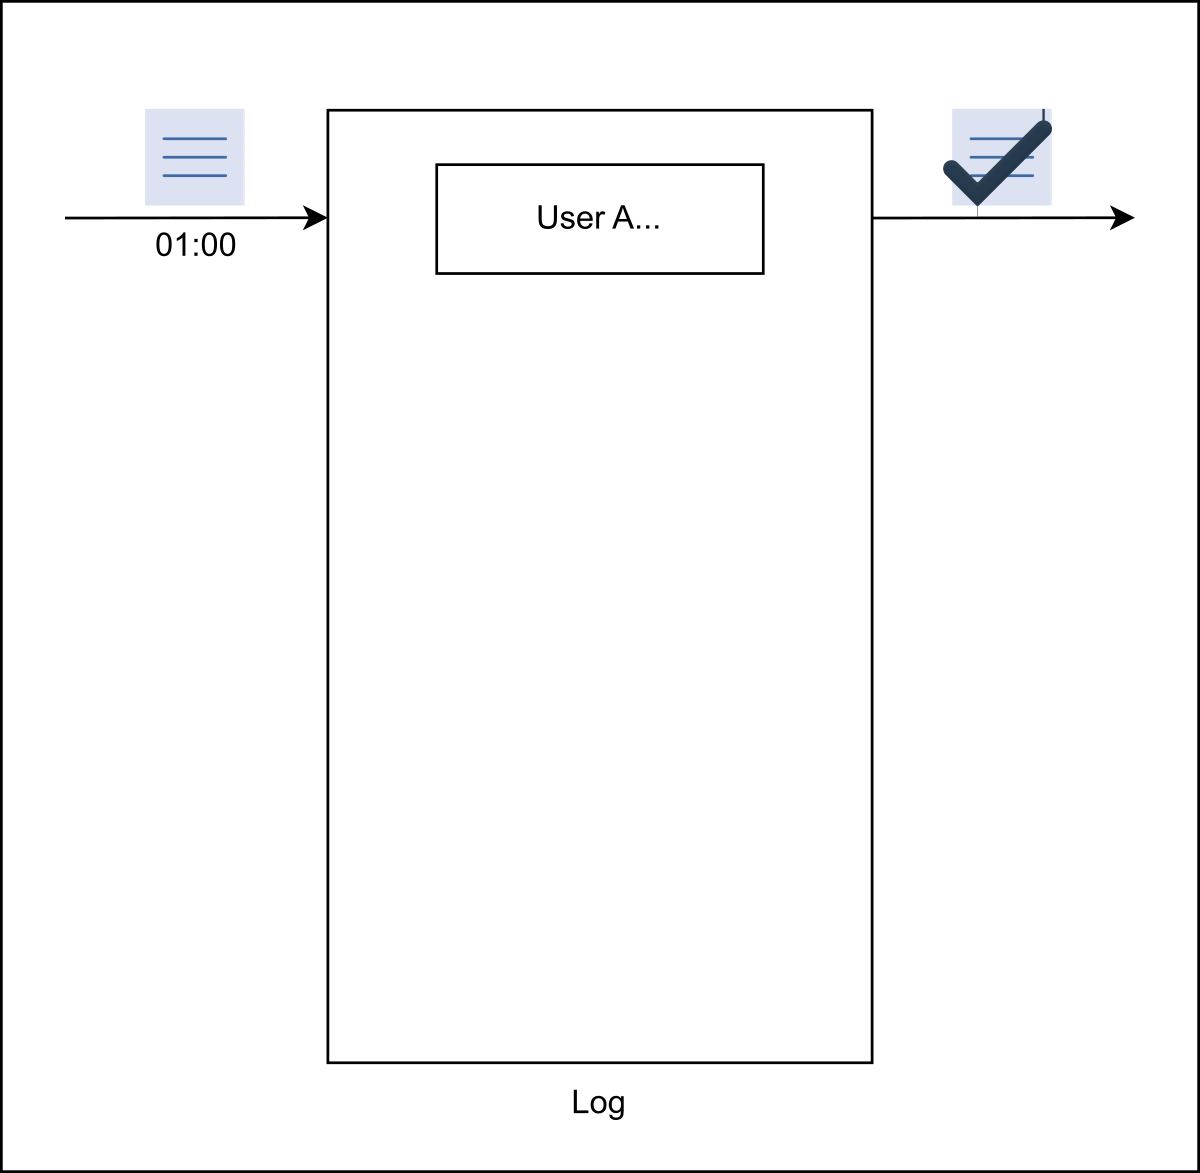
\includegraphics[width=\textwidth]{Images/chapter_19/section_5447913559293952/6080536686886912.png}
 \caption{A new request arrives at 01:00. Its arrival time is added to the log and the request is accepted. The time window is marked from 01:00 to 02:00}
 \end{subfigure}
 \hfill
 \begin{subfigure}[b]{0.48\textwidth}
 \centering
 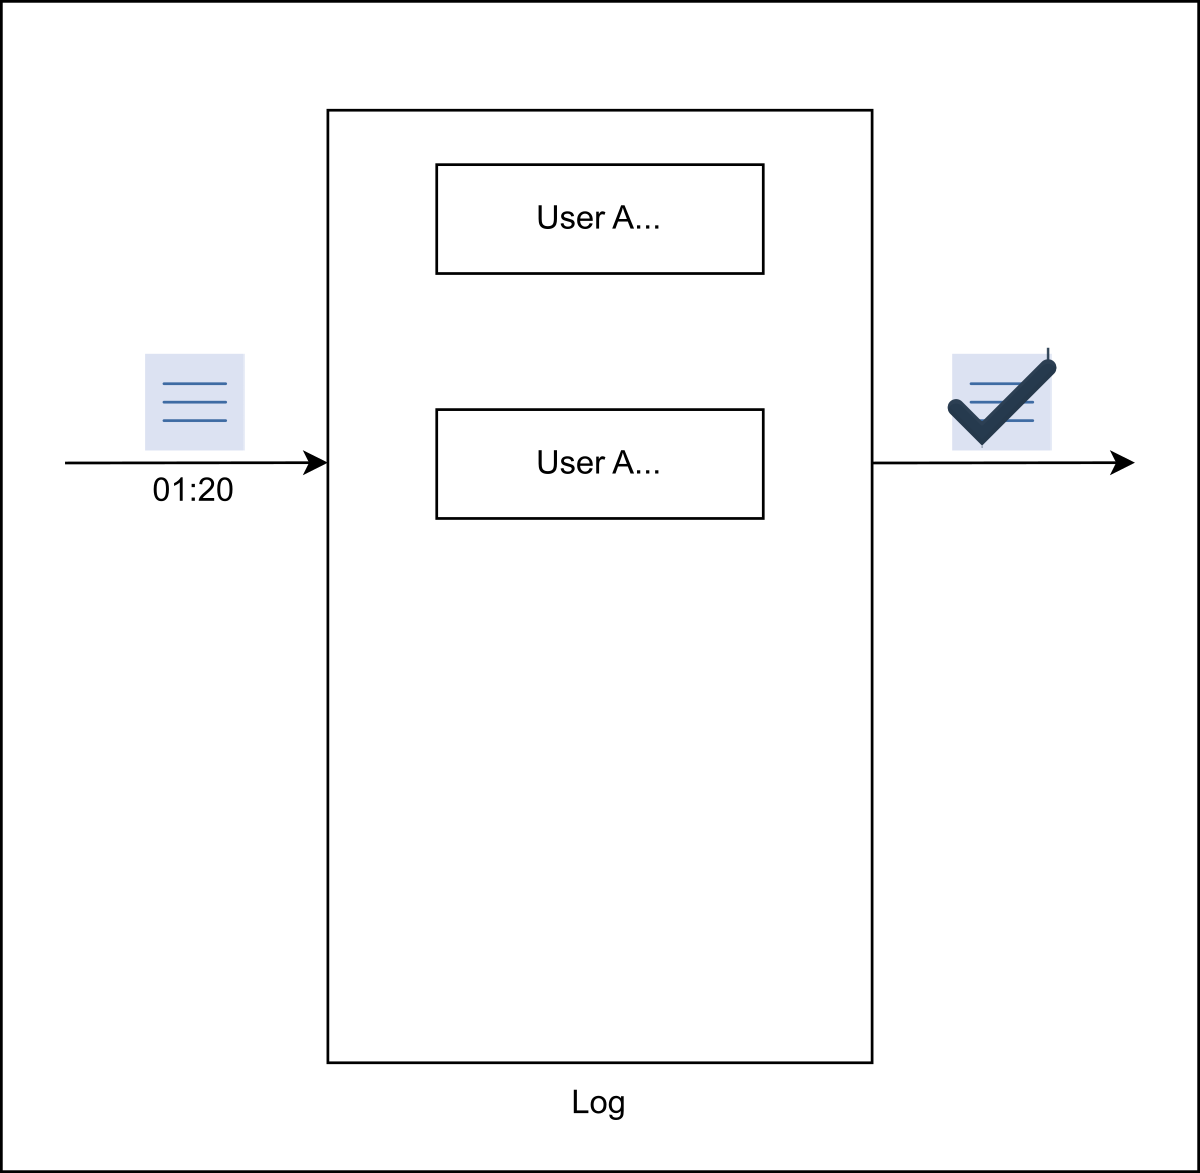
\includegraphics[width=\textwidth]{Images/chapter_19/section_5447913559293952/5540392103837696.png}
 \caption{Another request arrives at 01:20 and its timestamp is added to the log. As the log size is less than the maximum rate limit so it is allowed}
 \end{subfigure}
\end{figure}

\begin{figure}[htbp]
 \centering
 \begin{subfigure}[b]{0.48\textwidth}
 \centering
 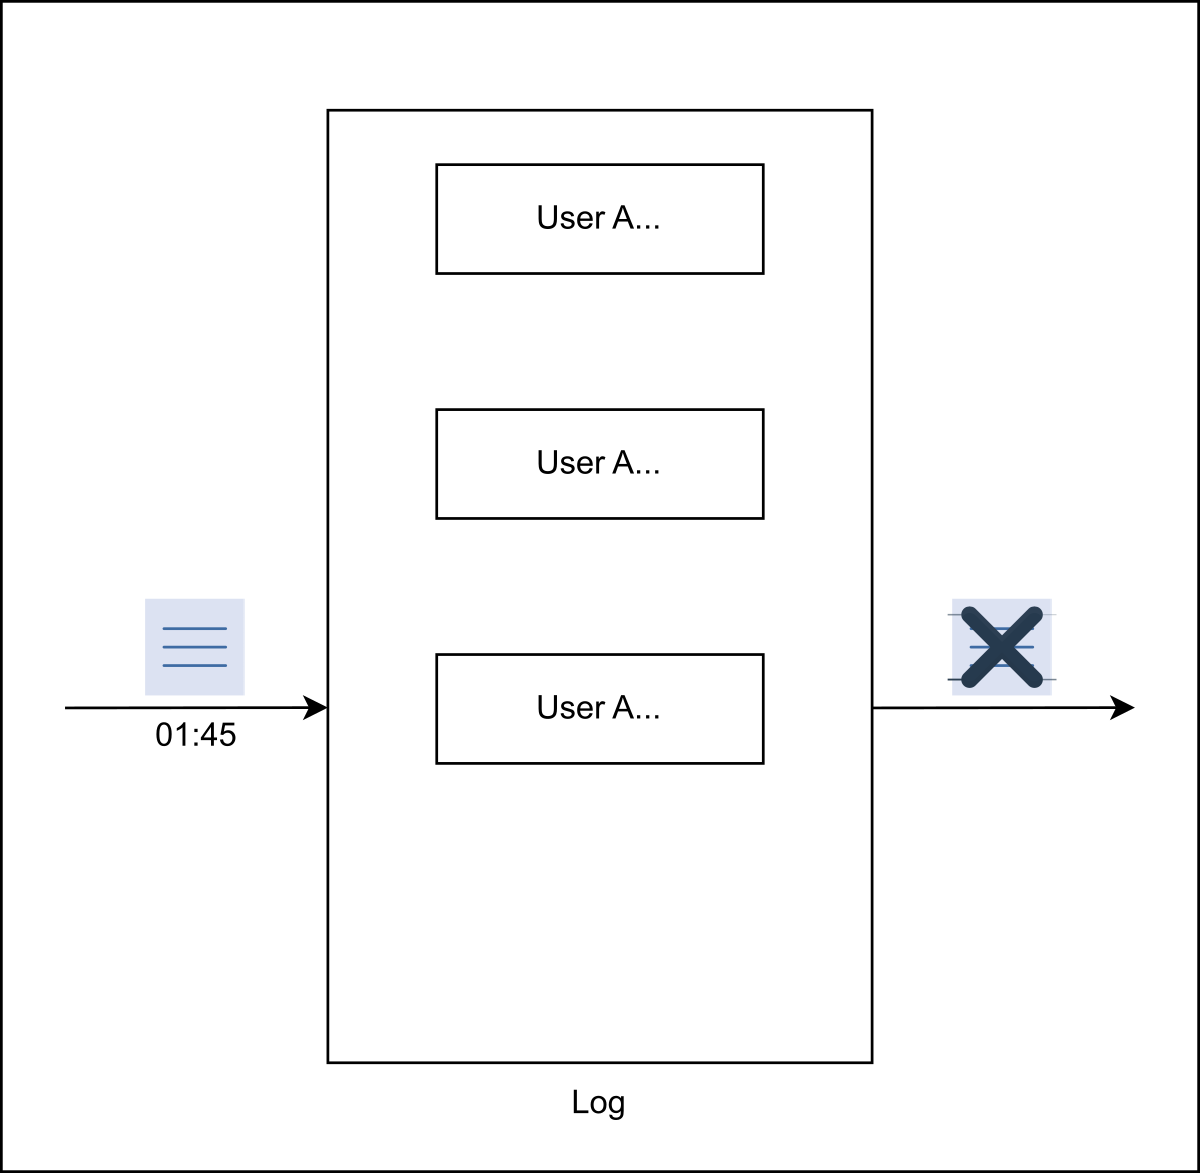
\includegraphics[width=\textwidth]{Images/chapter_19/section_5447913559293952/5241776684400640.png}
 \caption{The third request arrives at 01:45 and its timestamp is added to the log. The algorithm rejects the request because the log size becomes 3 which crosses the maximum limit }
 \end{subfigure}
 \hfill
 \begin{subfigure}[b]{0.48\textwidth}
 \centering
 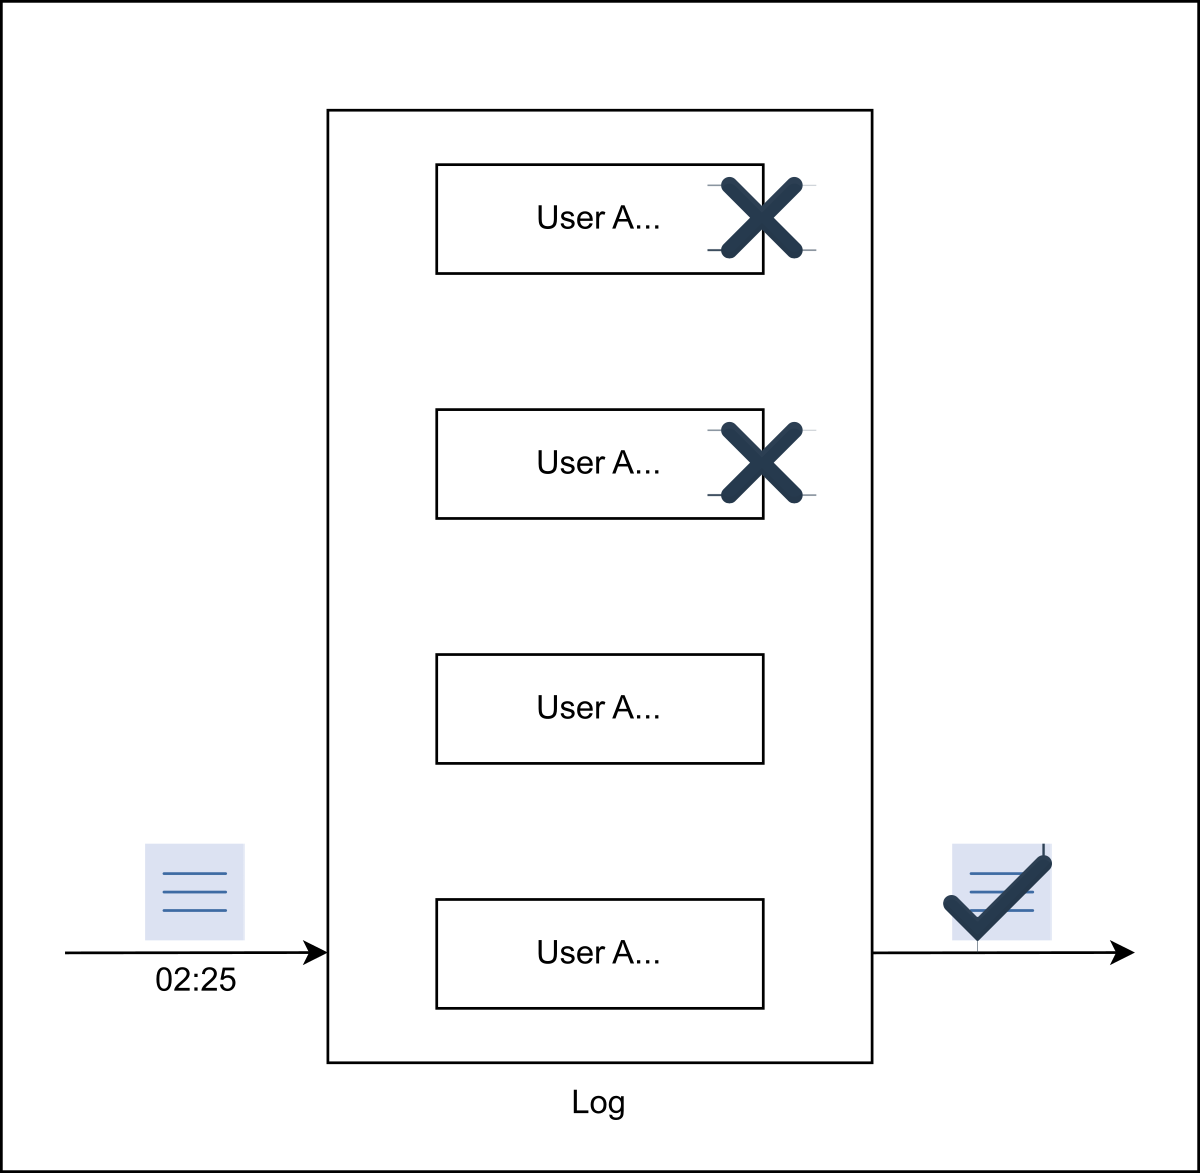
\includegraphics[width=\textwidth]{Images/chapter_19/section_5447913559293952/5493663597854720.png}
 \caption{A new request comes in at 02:25, and we start our new window from there. We keep one last window (from 01:25 to 02:25) in the log. The old data is removed from the log, and the size is reduced accordingly }
 \end{subfigure}
\end{figure}

\paragraph{Essential parameters}\label{nyt41-N941vp-X1jImPKP}
\\
The following parameters are required to implement the sliding window log algorithm:

\begin{itemize}
\item
\protect\phantomsection\label{l0w0f3pcNXPgPaEh5yaZZ}
\textbf{Log size} \protect\phantomsection\label{katex_inline_YwuL_UHvGEYy_agg8L-10}{{{\(\text{(L)}\)}}}\textbf{:} This parameter is similar to the rate limit (\protect\phantomsection\label{katex_inline_SX9al-owLiLO9mvKiysJh}{{{\(\text{R}\)}}}) as it determines the number of requests allowed in a specific time frame.
\item
\protect\phantomsection\label{qhcYswpTHHs4R6n47TQqo}
\textbf{Arrival time} \protect\phantomsection\label{katex_inline_40AKb6z_OddTq0d82OAEn}{{{\(\text{(T)}\)}}}\textbf{:} This parameter tracks incoming requests' time stamps and determines their count.
\item
\protect\phantomsection\label{5QAo5VIhqEBmzj1A39sTF}
\textbf{Time range} \protect\phantomsection\label{katex_inline_a0GZ6J0eNkl5j3enykJmq}{{{\(\text{(T}_\text{{r})}\)}}}\textbf{:} This parameter determines the time frame. The time stamps of the old requests are deleted if they do not fall in this range. The start time of the window is defined based on the first incoming request and expires after one minute. Similarly, when another request after the expiry time arrives the window ranges are updated accordingly.
\end{itemize}
\\
\paragraph{Advantages}\label{2Y_z1Sczrz_EkLAb4w4_5}

\begin{itemize}
\item
\protect\phantomsection\label{oC8jiwwA5g2pa95ZaRp3n}
The algorithm doesn't suffer from the boundary conditions of fixed windows.
\end{itemize}
\\
\paragraph{Disadvantages}\label{bwdPal1-F1X2zXWBfHRJZ}

\begin{itemize}
\item
\protect\phantomsection\label{fjYCxNJxISszFy5brs6wZ}
It consumes extra memory for storing additional information, the time stamps of incoming requests. It keeps the time stamps to provide a dynamic window, even if the request is rejected.
\end{itemize}

\subsubsection{Sliding window counter algorithm}\label{m93iAGcTftndadWfTwjwj}
\\
Unlike the previously fixed window algorithm, the \textbf{sliding window counter algorithm} doesn't limit the requests based on fixed time units. This algorithm takes into account both the fixed window counter and sliding window log algorithms to make the flow of requests more smooth. Let's look at the flow of the algorithm in the below figure.

\begin{figure}[htbp]
 \centering
 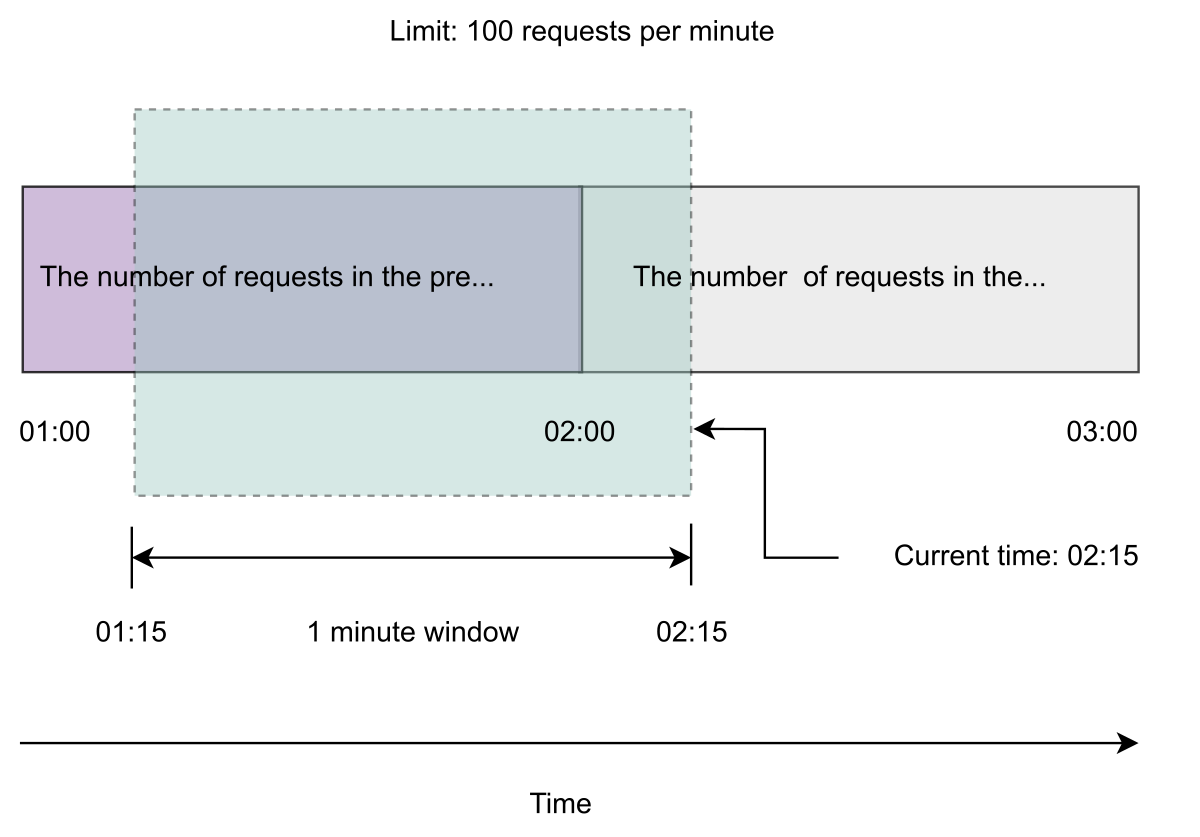
\includegraphics[width=0.5\textwidth]{Images/chapter_19/section_5447913559293952/6659323493351424.png}
 \caption{A sliding window counter algorithm, where the green shaded area shows the rolling window of 1 minute}
\end{figure}

In the above figure, we've 88 requests in the previous window while 12 in the current window. We 've set the rate limit to 100 requests per minute. Further
, the rolling window overlaps 15 seconds with the current window. Now assume that a new request arrives at 02:15. We 'll decide which request to accept or reject using the mathematical formulation:

\[
\text{Rate} = \text{R}_\text{{p}} \times \frac{\text{time frame} - \text{overlap time}}{\text{time frame}} + \text{R}_\text{{c}}
\]

Here, \protect\phantomsection\label{katex_inline_-aAKwD3Eh7r_ndwFMwkbT}{{{\(\text{R}_\text{{p}}\)}}}\hspace{0pt} is the number of requests in the previous window, which is 88. Rc R\_\{c\} Rc\hspace{0pt} is the number of requests in the current window, which is 12. The
\protect\phantomsection\label{katex_inline_sCsSN-zDNSE2BqUM_pfot}{{{\(\text{time frame}\)}}} is 60 seconds in our case, and \protect\phantomsection\label{katex_inline_0aYkLj1BNTEndZN1E-6ch}{{{\(\text{overlap time}\)}}} is 15 seconds.

\[
\text{Rate} = 88 \times \frac{60 - 15}{60} + 12
\]

\[
\text{Rate} = 78 < 100
\]

\paragraph{Essential parameters}\label{M0MFYVAxAvPT9_slBHeD_}
\\
This algorithm is relatively more complex than the other algorithms described above. It requires the following parameters:

\begin{itemize}
\item
\protect\phantomsection\label{K82RBE9s6c1TLINLCID3J}
\textbf{Rate limit} \protect\phantomsection\label{katex_inline_cr4jvMm8YCXKkylFND-Un}{{{\(\text{(R)}\)}}}\textbf{:} It determines the number of maximum requests allowed per window.
\item
\protect\phantomsection\label{QoM0wfX784qiHATMPukXX}
\textbf{Size of the window} \protect\phantomsection\label{katex_inline_TLIo6A7kNknttigHq3M58}{{{\(\text{(W)}\)}}}\textbf{:} This parameter represents the size of a time window that can be a minute, an hour, or any time slice.
\item
\protect\phantomsection\label{LhvkIaXHuJrx39CiG7L8E}
\textbf{The number of requests in the previous window} \protect\phantomsection\label{katex_inline_bwMjARGu4Q3-ddsDj6Qab}{{{\(\text{(R}_\text{{p}})\)}}}\textbf{:} It determines the total number of requests that have been received in the previous time window.
\item
\protect\phantomsection\label{4Zhq-1ni58RULfAk1dCqC}
\textbf{The number of requests in the current window} \protect\phantomsection\label{katex_inline_0D4FjGEUW9uF_Yj8JA5L-}{{{\(\text{(R}_\text{{c}})\)}}} \textbf{:} It represents the number of requests received in the current window.
\item
\protect\phantomsection\label{F5Voxv7FjBvpZmC7Vm4Ig}
\textbf{Overlap time} \protect\phantomsection\label{katex_inline_vrZWPbFADHcfGPj9l_vZj}{{{\(\text{O}_\text{{t}}\)}}} \textbf{:} This parameter shows the overlapping time of the rolling window with the current window.
\end{itemize}
\\
\paragraph{Advantages}\label{0zdVcY3Tv5Lw4ira5kc0T}

\begin{itemize}
\item
\protect\phantomsection\label{nYRD04w51FYGPBy4pu8XE}
The algorithm is also space efficient due to limited states: the number of requests in the current window, the number of requests in the previous window, the overlapping percentage, and so on.
\item
\protect\phantomsection\label{r9nwPJcgCC1p5NOISu-bn}
It smooths out the bursts of requests and processes them with an approximate average rate based on the previous window.
\end{itemize}
\\
\paragraph{Disadvantages}\label{Ti8Snk-2R1kbiu4ZOOm0i}

\begin{itemize}
\item
\protect\phantomsection\label{gegOJCIgGywy_BhRdNVBe}
This algorithm assumes that the number of requests in the previous window is evenly distributed, which may not always be possible.
\end{itemize}

\subsection{A comparison of rate-limiting algorithms}\label{Dg1pAYq16-L0ZxSS9suXu}
\\
The two main factors that are common among all the rate-limiting algorithms are:

\begin{itemize}
\item
\protect\phantomsection\label{bamUF__L5YYqAoEzcdaDf}
\textbf{Memory:} This feature refers to the number of states an algorithm requires to maintain for a normal operation. For example, if one algorithm requires fewer variables (states) than the other, it is more space efficient.
\item
\protect\phantomsection\label{6BbiCU0Q6YX3zQJR0lhKV}
\textbf{Burst:} This refers to an increase of traffic in a unit time exceeding the defined limit.
\end{itemize}
\\
The following table shows the space efficiency and burst of traffic for all algorithms that have been described in this lesson.

\textbf{A Comparison of Rate-limiting Algorithms}

\begin{table}[htbp]
\centering
\small
\adjustbox{max width=\textwidth}{
\begin{tabular}{|p{0.284\textwidth}|p{0.342\textwidth}|p{0.325\textwidth}|}
\hline
\textbf{Algorithm} & \textbf{Space efficient} & \textbf{Allows burst?} \\
\hline
\hline
Token bucket & Yes & Yes, it allows a burst of traffic within defined limit. \\
\hline
Leaking bucket & Yes & No \\
\hline
Fixed window counter & Yes & Yes, it allows bursts at the edge of the time window and can exceed the defined limit. \\
\hline
Sliding window log & No, maintaining the log requires extra storage. & Yes, it allows bursts when the window is empty or nearly empty, though it smooths out traffic as the window fills. \hfill\break \\
\hline
Sliding window counter & Yes, but it requires relatively more space than other space efficient algorithms. & Smooths out the burst \\
\hline
\end{tabular}
}
\caption{A Comparison of Rate-limiting Algorithms}
\end{table}

\begin{quote}
\textbf{Note:} Locking is not always bad by employing the above algorithms. If there is little contention on a lock, acquiring the lock takes little time. If we have high lock contention, a careful analysis is required to manage the situation, possibly by sharding the data and using multiple / finer-grained locks.
\end{quote}
\subsection{Conclusion}\label{P9YYpLdgT0p-eNCZJUvvB}
\\
In this lesson, we explored various popular rate-limiting algorithms. We also shed light on the advantages and disadvantages of these algorithms. Each of these algorithms can be deployed based on the user choice and the type of use case.

% End of section content